\documentclass[ aip, 12pt]{revtex4-1} % style for Physical Review B and AJP are similar
\usepackage{float}
\usepackage{amsmath}

\usepackage{graphicx} 


\usepackage{sverb}

\begin{document}

\title{Physics of Digital Data Storage}
\author{Tenzin Rigden}
\affiliation{Carleton College, Department of Physics, Northfield, MN 55057}
\date{\today}

\begin{abstract}
Word count: 
\end{abstract}

\maketitle
\section{Introduction}
On a fundamental level, a computer stores everything in a series of 1s or 0s called bits. Movies, pictures, and applications are all stored as a series of billions of these bits. In this binary system, 1 represents a true/on state while a 0 represents a false/off state. 
\section{Background}


\section{Optical Storage}
\subsection{Background}
Optical storage devices are devicecs that use optical methods to record and read information. For optical disks, data is recorded and read using a laser beam. To record data, a laser beam is shined on the reflective surface creating a pit with a depth of the wavelength of the laser divided by 2. Thus lands are the areas that were not shined on by the laser. To read, a very low power laser is shined on the disk and the reflected signal is converted to an electrical signal using a scanning photo detector. A "1" is interperted as when there is a change in the surface, i.e. changing from pit to land or land to pit, and a "0" is interperted as when there is no change in the surface. The way this is manifested is that when at a changing point for the surface, the laser will be shining at both the land and the pit. This means that the light reflected off of the pit will have a phase change of $\lambda/2$ behind the light reflected off of the land causing destructive interference and no reflected light, "1". When there is no change in the surface, the light simply reflects back normally and is interpreted as a "0." (CITE MEMORY MASS STORAGE)

\begin{figure}[H]
\centerline{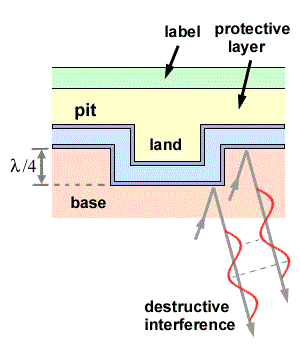
\includegraphics[scale=.9]{cdRom.png}}
\caption{ }
\label{cdRom}
\end{figure} 
\subsection{Optical Disks}
Optical Disks come in a few different styles: Compact Disk ROM (CD-ROM), CD-Recordable (CD-R), CD-Rewriteable (CD-RW), and Digital Versatile Disk (DVD). These disc technologies are written sequentially in a continous spiral track eminating from the middle out. This causes it to be slower than other technologies that use cocentric tracks. A CD-ROM is a disc that's only meant to be readable and typically used for things such as installation of programs. Since it is only written once in the factory, a glass master disk is created using a high intensity laser. Liquid polycarbonate is inserted into the master disk to recreate the disk which is then covered with a reflective layer then a protective one. 
A CD-R is slightly different because it needs to be able to written to once outside of the factory. This is one by having a painted layer between the reflective layer and transparent layer. The painted layer is initially transparent and becomes dark to simulate a pit when impacted by a high-intensity laser. Lastly, in a CD-RW, the reflective layer has two states, a slightly reflective amorphous state and a highly reflective crystalline state. A high intensity laser shined on this layer will cause it to turn into its amorphous state and simulates a pit, while a medium intensity laser will cause it to change back into its crystalline state and simulates a land. And again, a low intensity laser is used to read the pits and lands without affecting the state.

\begin{figure}[H]
\centerline{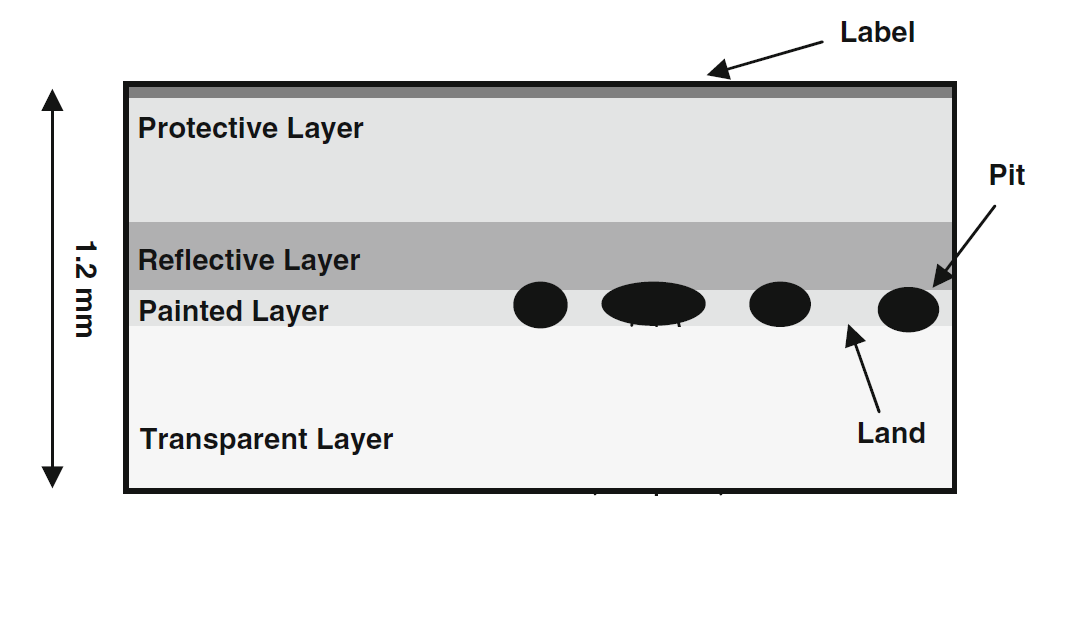
\includegraphics[scale=.45]{cdR.png}}
\caption{ }
\label{cdR}
\end{figure} 

While CDs were useful and easy to carry around, their size was limited to only 700MB. Demand for higher storage capacities in the 1990s led to the invention of the DVD which offered data storage of at least 4.7GB. The first main difference between CDs and DVDs is that DVDs use a shorter wavelength light, 650nm, than CDs use, 780nm. What this allows is that pits and lands in the DVD are much smaller and can be placed closer together than a CD could, increasing storage density. Another innovation that allowed storage of up to 8.5GB was the ability to have two different recording layer: a semi reflective layer in the middle and a fully reflective layer at the other end. The different layers can be read by changing the focus of the laser. Additionally, instead of having a protective layer on one side of the disk, you can put another disc on it to effectively double the capacity again. However, this requires the manual flipping of the disc when accessing the other half of the data. By having double sided and a double layer, DVDs can achieve a storage of 17GB.

\begin{figure}[H]
\centerline{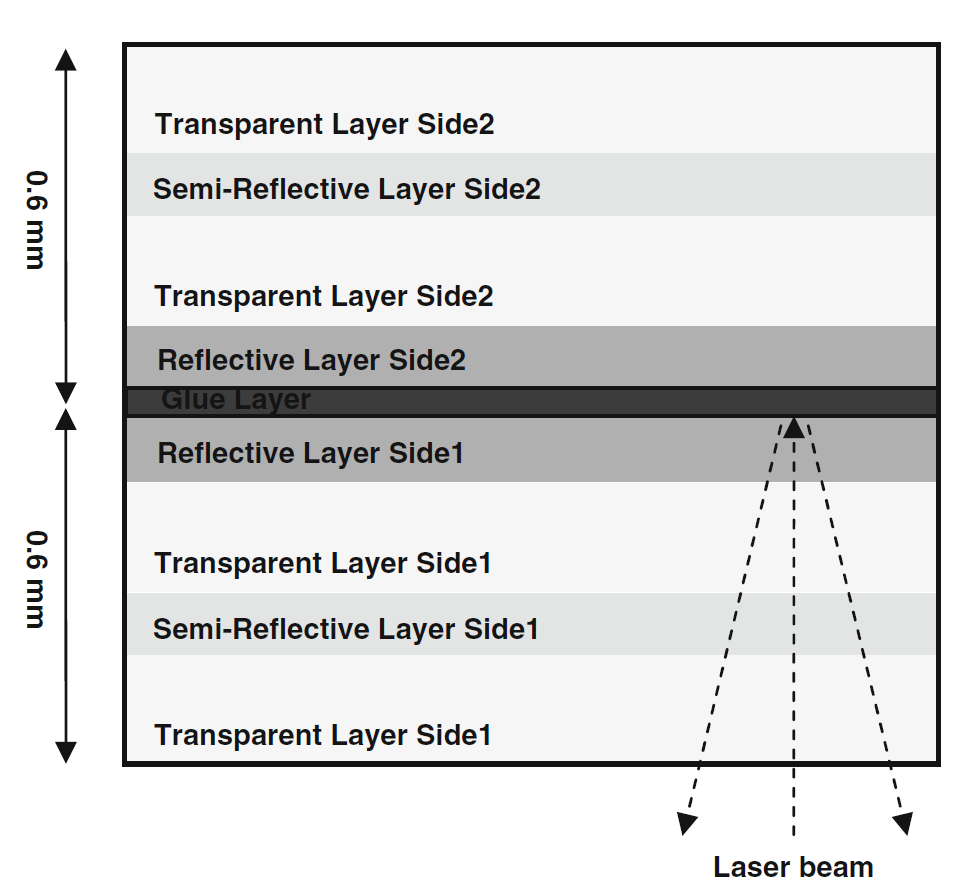
\includegraphics[scale=.45]{DVD.png}}
\caption{ }
\label{DVD}
\end{figure} 


\section{Magnetic Storage}
\subsection{Background}
Magnetic storage is a property can be attributed to the ferromagnetic property of certain metals such as iron and cobalt. Ferromagnetic materials are divided into small magnetic domains each with their own magnetic field in a direction. An unmagnetized ferromagnet will have these domains in random directions such that the net effect is 0 as seen in figure \ref{domain}a. However, if an external magnetic field is applied, these domains will align with the external field and will stay aligned even after the external field is removed as in figure \ref{domain}b. 

\begin{figure}[H]
\centerline{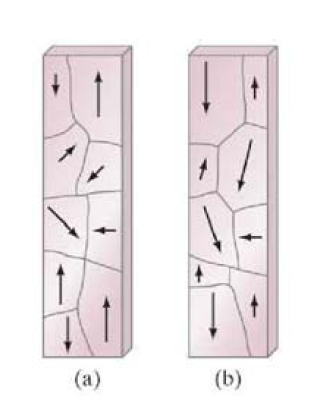
\includegraphics[scale=.45]{magneticDomain.png}}
\caption{ }
\label{domain}
\end{figure} 
This is due to the hysteresis loop experienced by the ferromagnetic material. If we start with an unmagnetized ferromagnetic material with no external magnetic field, point a in figure \ref{hysteresis}, and increase the external magnetic field, $B_0$, we get to point b where there is a both a nonzero external amgnetic field and total field from the external and material. If the external magnetic field is then decreased to zero, instead of returning to point a, it instead reaches point c. Here, even though there is no external magnetic field, there is still an internal field from the ferromagnetic material. This phenomenom is what allows magnetic storage to store bits. Aligning a certain domain's magnetic field in one direction can signify a 1 while the other direction's signifies a 0.


\begin{figure}[H]
\centerline{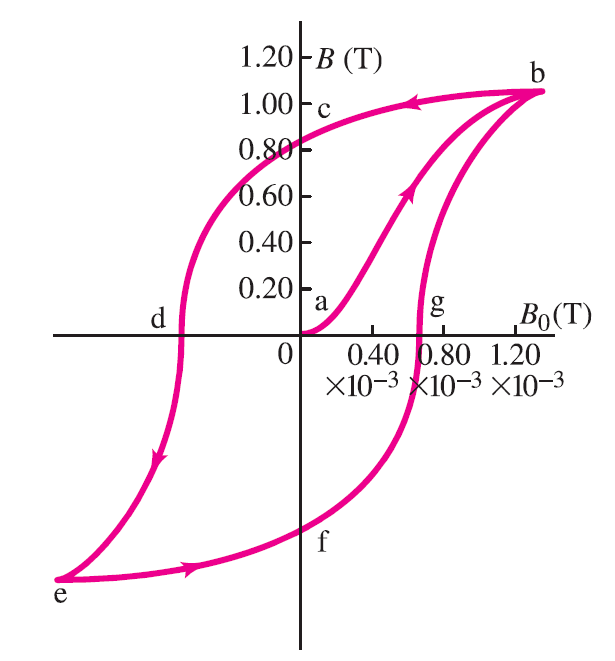
\includegraphics[scale=.45]{hysteresis.png}}
\caption{ }
\label{hysteresis}
\end{figure}

Reading and writing to the material is done by inducing a magnetic field using a head and coil of wire. The mechanics behind this are governed by Maxwell's equations. The two relevant equations are
\begin{equation}
\nabla x E = -\frac{\partial B}{\partial t},
\label{faraday}
\end{equation}
which is known as Faraday's law of induction and 
\begin{equation}
\nabla x B = \mu_0 J +\mu_0\epsilon_0\frac{\partial E}{\partial t},
\label{ampere}
\end{equation}
which is known as Ampere's law (cite purcell). Faraday's law tells us that a changing electric field will yield and changing magnetic field, and Ampere's law tells us the opposite. 

\subsection{Magnetic Disk Storage}
A magnetic disk drive is the most commonly used data storage technology used in consumer products today. First introduced in 1956 by IBM, modern drives consist of mainly of a read/write head and a hard platter with a ferromagnetic layer. Originally, the head was used for both reading and writing but compromises had to be made. The read head wants a thicker gap to be better able to penetrate the medium while the write head wants a smaller gap to get better accuracy. As domains got smaller, it became more and more difficult for the read/write heads to be able to properly read the intended domain from the increasing noise of the other domains. Nowadays, reading is done instead by a giant magnetoresistive (GMR) head. Magnetoresistance (MR) is the property that when a coiled wire will not only generate an electric field/current, it will also experience a change in resistance. This change in resistance can be used as a more accurate way to read the bits by applying a constant potential across a MR sensor and recording how the potential changes due to the change in the resistance of the wire because of Ohm's law. GMR is similar to MR but actually is a quantum effect. It is appropriately named because of its ability to change the resistance is giant in comparison to MR.  (CITE HIGH DENSITY DATA STORAGE) 

TALK MORE ABOUT GMR
The mechanism behind this goes goes into the spin state of the moving electrons. These electrons can only have one of two possible states, up or down. If the spin states align with the direction of the magnetic field, they move forward in the wire simulating a lower resistance. However, if the spin state is against the field, then the electrons will travel in the opposite direction of the current causing more collisions and thereby increasing the resistance of the wire. (CITE HIGH DENSITY DATA STORAGE)

The innovation of GMR read head and a dedicated write head allowed the domain bits to shrink even more. However, a new issue began to arise. The ability to retain stored data in the material is dependent on the product of $K_u$ and $V$ where $K_u$ is the magnetic anisotropy constant of the material. This product gives the energy barrier that must be overcome that allows the material to keep its magnetic field even without the external field. However, as the domains decrease in size to increase density, the volume decreases and so does the energy barrier. If the volumte of the domain decreases to the point where this energy barrier is on the same order of magnitude as thermal energy, $K_bT$, the domain may randomly switch its field direction and "flip bits." This created a limit to the storage density that longitudinal recording could attain.(CITE PERPENDICULAR RECORDING ARTICLE)

To surpass this limit, the orientation of the recorded magnetic field changed from longitudinal recording to perpendicular recording. In addition to the change in orientation, the writing head was changed to a single-pole head and a highly permeable soft underlayer(SUL) was added below the recording material. The permeability of the SUL allowed it to act as a magnetic mirror to the actual head. This greatly increased the induced magnetic field used to write data. The stronger magnetic field means that materials with higher anisotropy values could be used that were not feasible for the weaker magnetic field in longitudinal recording. Because the anisotropy constant can be increased, the volume of the domain can be decreased further without worrying about thermal fluctuations.

\begin{figure}[H]
\centerline{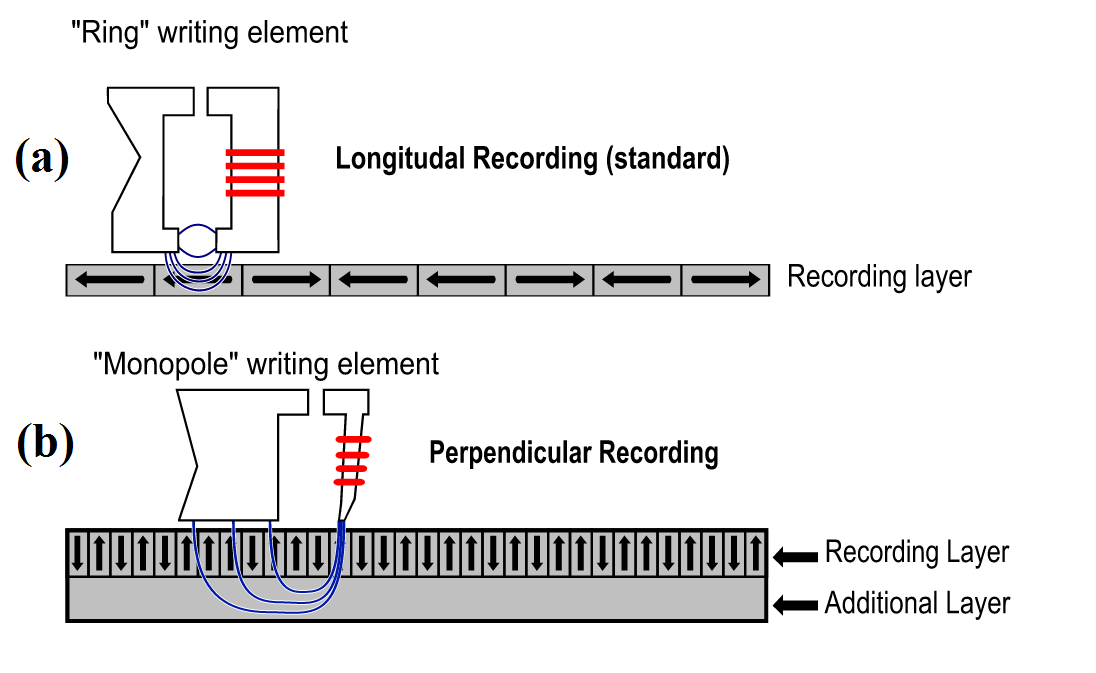
\includegraphics[scale=.45]{perpendicularComparison.png}}
\caption{ }
\label{perpendicularComparison}
\end{figure}


However, this too will have a limit at a smaller domain size where thermal fluctuations will be an issue again. One method still currently in development is called heat-assisted magnetic recording (HAMR). This method is based on the fact that all ferromagnetic materials have a curie temperature where the internal magnetic field it had is reduced to zero, and in the presence of an external magnetic field will align itself to that. In HAMR, when something needs to get written, a laser is used to heat up the desired domain to the curie temperature allowing our magnetic field to allign the domain, and then allowing the material to cool back down. This means that the recording material can be changed to one with a much higher anisotropy value allowing the domain sizes to decrease even more, further increasing the storage density. (CITE HAMR ARTICLE)


\section{Applications}
\subsection{Colloids}


\subsection {Optical Thermal Ratchets}


\subsection{Molecular Motors}

\section{Broader Impacts}


\bibliography{compsNotes}
\bibliographystyle{aip}


\end{document}
